\documentclass[11pt,a4paper]{article}

\usepackage[utf8]{inputenc}
\usepackage[T1]{fontenc}
\usepackage[french]{babel}
\usepackage{lmodern}
\usepackage{microtype}
\usepackage[margin=2.4cm]{geometry}
\usepackage{booktabs}
\usepackage{tabularx}
\usepackage{array}
\usepackage{xcolor}
\usepackage{enumitem}
\usepackage{float}
\usepackage{graphicx}
\usepackage{amsmath}
\usepackage{pifont}
\usepackage[round,authoryear]{natbib}
\usepackage[colorlinks=true,linkcolor=teal!70!black,citecolor=teal!70!black,urlcolor=teal!70!black]{hyperref}

\newcolumntype{Y}{>{\raggedright\arraybackslash}X}
\newcolumntype{C}[1]{>{\centering\arraybackslash}p{#1}}
\newcommand{\oui}{\textcolor{teal!70!black}{\ding{51}}}
\newcommand{\non}{\textcolor{red!60!black}{\ding{55}}}
\newcommand{\partiel}{\textcolor{orange!80!black}{$\sim$}}
\setlist{itemsep=2pt,topsep=4pt}

\title{\textbf{Router par la preuve et s'abstenir à temps :\\ allocation adaptative du calcul et de la
recherche documentaire pour des LLM locaux}\\[6pt]
\large Une évaluation pré-enregistrée de la qualité, de la latence et de l'énergie sur un ordinateur personnel}
\author{Alae Lahbichi\\[2pt]
\small Étudiant en 5\textsuperscript{e} année, Intelligence artificielle et science des données\\
\small\href{mailto:a.lahbichi2004@gmail.com}{\texttt{a.lahbichi2004@gmail.com}}\\
\small Code et données : \href{https://github.com/AlaeLahbichi/Adaptive-Compute-and-RAG-for-Efficient-Reliable-Local-LLMs}{\footnotesize\texttt{github.com/AlaeLahbichi/Adaptive-Compute-and-RAG-for-Efficient-Reliable-Local-LLMs}}}
\date{Octobre 2026}

\begin{document}
\maketitle

\begin{abstract}
\noindent Faire tourner un modèle de langage sur sa propre machine, c'est garder la maîtrise de ses
données, mais c'est aussi payer chaque réponse en secondes d'attente et en joules. Toutes les questions
ne méritent pourtant pas le même effort : certaines se règlent sans aucun document, d'autres demandent
un modèle plus puissant et plusieurs passages, d'autres encore n'ont pas de réponse dans le corpus, et
la seule réponse honnête est alors de s'abstenir. Cet article étudie comment prendre ces trois décisions
ensemble, question par question, à partir de signaux qui ne coûtent presque rien. Nous proposons une
politique qui s'appuie sur la suffisance des preuves, mesurée par le score BM25 du meilleur passage, et
sur la confiance du modèle, lue dans les probabilités des tokens qu'il produit. Nous l'évaluons sur un
Apple M3 Pro avec deux modèles Qwen quantifiés en 4 bits, sur un benchmark de 630 questions construit à
partir de SQuAD 2.0 et HotpotQA, en fixant les critères de succès avant toute expérience et en
n'exécutant le jeu de test qu'une seule fois. Sur 450 questions de test, la politique égale la qualité
de la configuration de référence (score de 0,550 contre 0,537, non-infériorité démontrée), commet moins
d'erreurs et devance deux routeurs inspirés de la littérature. Elle ne réduit cependant la latence que
de 10~\% et l'énergie de 9~\%, quand nous visions 20~\% : le critère principal n'est pas atteint. Nous
montrons que cet écart tient au réglage d'un seuil absolu sur un échantillon trop petit, et nous en
tirons un programme d'améliorations précis.

\medskip
\noindent\textbf{Mots-clés :} modèles de langage locaux, routage de modèles, RAG adaptatif, abstention,
sobriété énergétique, évaluation pré-enregistrée.
\end{abstract}

%======================================================================
\section{Introduction}\label{sec:intro}
%======================================================================

\subsection{Contexte}

Il y a encore peu, interroger un grand modèle de langage supposait d'envoyer sa question à un serveur
distant. Ce n'est plus le cas. Des modèles de quelques milliards de paramètres, une fois quantifiés,
tiennent dans la mémoire d'un ordinateur portable et y répondent en moins d'une seconde. Cette
évolution change la nature du problème. Une entreprise qui veut interroger ses archives sans les
confier à un tiers, un chercheur qui travaille sur des données sensibles, un étudiant qui n'a pas de
budget pour une API : tous peuvent désormais disposer d'un assistant local. En contrepartie, le coût de
chaque réponse cesse d'être une ligne abstraite sur une facture. Il devient du temps d'attente, de la
mémoire occupée, de la batterie consommée.

Deux leviers permettent d'améliorer les réponses d'un tel système, et tous deux ont un prix. Le premier
est la taille du modèle : un modèle plus grand raisonne mieux, mais il est plus lent. Le second est la
recherche documentaire, ou génération augmentée par récupération (RAG) : en joignant à la question des
passages extraits d'un corpus, on ancre la réponse dans des sources et l'on réduit les inventions du
modèle \citep{gao2023ragsurvey}. Mais chaque passage ajouté allonge le texte que le modèle doit lire, et
donc le temps de calcul. Il existe enfin une troisième issue, souvent oubliée : ne pas répondre.
Lorsque les documents ne contiennent pas l'information demandée, une abstention franche vaut mieux
qu'une réponse plausible et fausse \citep{wen2024abstention}.

\subsection{Problématique}

La pratique courante consiste à fixer une configuration une fois pour toutes, par exemple « le plus
grand modèle disponible avec trois passages », et à l'appliquer à toutes les questions. Ce choix est
confortable, mais il est doublement inefficace. Sur une question simple, dont la réponse figure en
toutes lettres dans un passage, il mobilise un modèle surdimensionné. Sur une question à laquelle le
corpus ne répond pas, il dépense une génération complète pour produire, au mieux, un aveu d'ignorance
et, au pire, une erreur. À l'inverse, choisir systématiquement la configuration la plus légère sacrifie
la qualité sur les questions difficiles.

Le problème est donc un problème d'\emph{allocation} : il s'agit de donner à chaque question les
ressources dont elle a besoin, ni plus ni moins. Il est délicat pour trois raisons. D'abord, il faut
décider \emph{avant} de connaître la réponse, à partir d'indices imparfaits. Ensuite, ces indices ont
eux-mêmes un coût : un signal de décision qui demande une génération supplémentaire peut annuler
l'économie qu'il est censé produire. Enfin, l'objectif est multiple. On veut réduire la latence et
l'énergie, mais sans perdre en qualité, sans augmenter les erreurs et sans sacrifier une catégorie de
questions au profit d'une autre. Nous formulons ainsi la problématique de ce travail :

\begin{quote}
\emph{Comment allouer automatiquement, et de manière mesurable, les ressources de calcul et de recherche
documentaire à chaque requête, afin de réduire le coût d'un système de questions-réponses local sans
dégrader significativement la qualité, la factualité et la fiabilité de ses réponses ?}
\end{quote}

\subsection{Questions de recherche}

Cette problématique se décline en quatre questions, qui structurent la suite de l'article.

\begin{description}[style=sameline,leftmargin=1.2cm]
\item[QR1] Peut-on, à partir d'un signal peu coûteux, choisir le modèle et le niveau de recherche
documentaire sans perte de qualité ?
\item[QR2] Peut-on décider de manière fiable quand s'abstenir, en combinant l'incertitude du modèle et
la qualité des preuves retrouvées ?
\item[QR3] Quel compromis entre qualité, latence et énergie obtient-on réellement sur un ordinateur
personnel, une fois compté le coût des signaux de décision ?
\item[QR4] Les gains sont-ils homogènes selon le type de question, ou certains profils sont-ils
sacrifiés ?
\end{description}

\subsection{Démarche et contributions}

Nous avons abordé ces questions par étapes, en nous imposant une discipline expérimentale stricte. Une
revue de la littérature a d'abord permis de situer le problème et de formuler des hypothèses. Nous avons
ensuite construit un benchmark et un protocole, puis écrit nos critères de succès \emph{avant} la
moindre expérience. Une étude pilote a validé la chaîne de mesure. Des méthodes de référence, fixes ou
inspirées de travaux publiés, ont fixé la barre. Nous avons alors conçu et réglé une politique
adaptative sur un jeu de développement, avant de la figer et de l'évaluer une seule fois sur un jeu de
test jamais consulté. Ce travail apporte cinq contributions :

\begin{enumerate}
\item une synthèse de la littérature qui montre que le choix du modèle, la décision de recherche et
l'abstention sont presque toujours traités séparément, avec un coût rarement mesuré sur matériel local ;
\item un benchmark et un protocole pré-enregistrés, avec mesure de la latence sur trois passes et de
l'énergie par \texttt{powermetrics} ;
\item un ensemble de méthodes de référence : six stratégies fixes et deux routeurs inspirés de RouteLLM
et d'Adaptive-RAG ;
\item une politique adaptative conjointe, simple et interprétable, fondée sur des signaux quasi gratuits ;
\item une évaluation finale dont nous rapportons honnêtement le résultat, partiellement négatif, avec
l'analyse de ses causes et des pistes d'amélioration concrètes.
\end{enumerate}

\paragraph{Organisation de l'article.} La section~\ref{sec:cadre} définit les notions employées. La
section~\ref{sec:etat} présente l'état de l'art et en déduit nos hypothèses. La
section~\ref{sec:protocole} décrit le benchmark et le protocole, la section~\ref{sec:pilote} l'étude
pilote, la section~\ref{sec:references} les méthodes de référence et la section~\ref{sec:politique} la
politique adaptative. La section~\ref{sec:final} rapporte l'évaluation finale. Nous discutons ces
résultats en section~\ref{sec:discussion}, examinons les faiblesses de l'étude en
section~\ref{sec:faiblesses}, et concluons en section~\ref{sec:conclusion}.

%======================================================================
\section{Cadre conceptuel}\label{sec:cadre}
%======================================================================

Plusieurs termes reviennent tout au long de cet article. Nous les précisons ici, car leur usage varie
d'un travail à l'autre.

On appelle \textbf{routage} le fait de choisir, avant toute génération, le modèle qui traitera une
requête parmi plusieurs candidats de tailles ou de coûts différents. La \textbf{cascade} en est une
variante séquentielle : on interroge d'abord un modèle peu coûteux, puis on passe la main à un modèle
plus puissant si la première réponse paraît peu fiable. Le coût du premier modèle est alors payé dans
tous les cas, ce qui pèse lourd lorsque l'escalade est fréquente.

La \textbf{génération augmentée par récupération} (RAG) consiste à ajouter au prompt des passages
extraits d'une base documentaire. Le RAG est dit \textbf{adaptatif} lorsqu'il décide, requête par
requête, s'il faut chercher, quand chercher et combien de passages retenir.

L'\textbf{incertitude} désigne une estimation de la probabilité qu'une réponse soit fausse. Elle peut
se lire dans les probabilités internes du modèle, dans la cohérence entre plusieurs réponses
échantillonnées, ou dans la confiance que le modèle exprime lui-même. Les \textbf{preuves} sont les
passages retrouvés ; leur \textbf{suffisance} mesure dans quelle mesure ils semblent contenir de quoi
répondre.

L'\textbf{abstention} est le refus de répondre lorsque le risque d'erreur est jugé trop élevé. On
l'évalue par deux grandeurs complémentaires \citep{kamath2020selective} : la \textbf{couverture}, part
des questions auxquelles le système répond, et le \textbf{risque}, part des réponses fausses parmi
celles qu'il donne. S'abstenir davantage fait baisser la couverture ; c'est utile si le risque baisse
en proportion.

Enfin, le \textbf{coût} n'a pas le même sens partout. Selon les travaux, il s'agit du prix facturé par
une API, du nombre d'appels au grand modèle, du nombre de tokens, de la latence, de la mémoire ou de
l'énergie. Ces mesures ne sont pas interchangeables. Dans ce travail, le coût est celui que subit
l'utilisateur d'une machine personnelle : la latence de bout en bout et l'énergie consommée par la
puce, complétées par le nombre de tokens.

%======================================================================
\section{État de l'art}\label{sec:etat}
%======================================================================

\subsection{Méthode de revue}

Nous avons interrogé arXiv, ACL Anthology, OpenReview, Google Scholar et Semantic Scholar, ainsi que
les actes de NeurIPS, ICLR, AAAI et MLSys. Les requêtes croisaient les notions du sujet et leurs
synonymes anglais : \textit{LLM routing}, \textit{model cascade}, \textit{adaptive retrieval},
\textit{adaptive RAG}, \textit{uncertainty estimation}, \textit{selective prediction},
\textit{abstention} et \textit{energy-aware inference}. Nous avons retenu les travaux qui adaptent,
requête par requête, le choix du modèle, la recherche documentaire ou la décision de répondre, à
condition qu'ils s'accompagnent d'une évaluation expérimentale, ainsi que les études de coût
d'inférence et les jeux de données utiles à notre protocole. Les travaux d'infrastructure, les articles
de position sans expérience et les systèmes multi-agents hors du cadre des questions-réponses ont été
écartés. Partis de dix-sept références, nous en avons identifié cinquante et une en suivant les
citations dans les deux sens et en menant une recherche ciblée sur les travaux de 2025 et 2026 ;
quarante-six ont été retenues et classées par thème.

\subsection{Routage et cascades de modèles}

L'idée de réserver le grand modèle aux requêtes qui le justifient est ancienne, mais elle a pris de
l'ampleur avec la multiplication des API payantes. \citet{chen2023frugalgpt} en donnent une formulation
générale avec FrugalGPT, qui enchaîne des modèles de coût croissant et s'arrête dès qu'un évaluateur
appris juge la réponse acceptable ; ils rapportent des économies considérables à qualité égale. AutoMix
\citep{aggarwal2023automix} remplace cet évaluateur par une auto-vérification du petit modèle, dont le
bruit est absorbé par un processus de décision markovien. \citet{yue2023cascades} utilisent un autre
indice : lorsque plusieurs réponses du petit modèle concordent, il y a de bonnes chances qu'il ait
raison.

Une seconde famille décide \emph{avant} toute génération. Hybrid LLM \citep{ding2024hybrid} prédit la
difficulté d'une requête pour l'envoyer au petit ou au grand modèle, avec un seuil réglable au moment de
l'inférence. RouteLLM \citep{ong2024routellm} apprend ce choix à partir de préférences humaines et montre
que les routeurs obtenus se transfèrent à d'autres paires de modèles. D'autres travaux recourent à un
bandit manchot \citep{nguyen2024metallm} ou à un modèle de récompense \citep{lu2023zooter}. Pour
comparer ces approches, RouterBench \citep{hu2024routerbench} propose un cadre d'évaluation commun.

Les travaux les plus récents affinent la notion de coût et de garantie. \citet{fu2026inflation}
montrent que le coût d'un appel isolé sous-estime largement celui d'un processus qui relance les
requêtes, et proposent un signal de difficulté calculé localement avant exécution. RACER
\citep{hao2026racer} produit des ensembles de modèles avec un seuil calibré qui autorise l'abstention et
contrôle le risque d'erreur de routage, avec des garanties qui ne supposent rien de la distribution des
données. La revue de \citet{varangot2025survey} dresse un bilan du domaine et en souligne deux faiblesses
: des protocoles expérimentaux peu standardisés et une prise en compte quasi exclusive du coût
financier.

\subsection{RAG adaptatif}

Que la recherche documentaire ne soit pas toujours utile, \citet{mallen2022trust} l'ont montré de façon
convaincante : les modèles retiennent bien les connaissances populaires et mal les connaissances rares,
si bien que récupérer seulement lorsque c'est nécessaire améliore à la fois la précision et le coût. Les
méthodes qui ont suivi diffèrent surtout par l'indice qui déclenche la recherche. SKR
\citep{wang2023skr} s'appuie sur ce que le modèle sait de lui-même ; FLARE \citep{jiang2023flare} et
DRAGIN \citep{su2024dragin} déclenchent la recherche en pleine génération, dès que le modèle hésite ;
Self-RAG \citep{asai2023selfrag} apprend au modèle à émettre des jetons de réflexion qui jugent la
pertinence des passages, au prix d'un entraînement dédié.

Adaptive-RAG \citep{jeong2024adaptiverag} est la référence la plus proche de notre problème. Un petit
classifieur y prédit la complexité de la question et choisit entre aucune recherche, une recherche en
une étape et une recherche itérative. HyPA-RAG \citep{kalra2024hyparag} transpose cette idée aux
paramètres de recherche dans le domaine juridique. D'autres travaux jugent plutôt les documents que la
question : Corrective RAG \citep{yan2024crag} évalue les passages retrouvés et décide de les utiliser,
de les compléter ou de les écarter, et Tiny-Critic RAG \citep{wu2026tinycritic} confie ce contrôle à un
petit modèle pour en réduire la latence.

Une étude comparative de \citet{moskvoretskii2025adaptive} a particulièrement orienté notre travail : sur
une trentaine de méthodes, des estimateurs d'incertitude simples rivalisent avec des pipelines bien plus
complexes, et les dépassent souvent en efficacité. Plus récemment, Self-Routing RAG \citep{wu2025srrag}
traite le modèle lui-même comme une source de connaissance parmi d'autres, RAGRouter-Bench
\citep{wang2026ragrouterbench} formule le choix d'un paradigme de RAG comme un problème de routage, et
Pre-Route \citep{chen2026preroute} arbitre entre RAG et contexte long. Enfin, plusieurs travaux
réduisent le coût du contexte lui-même, en ne conservant que les phrases utiles
\citep{arefeen2024leancontext,akesson2024clustered,chen2026logicrag}.

\subsection{Incertitude et abstention}

Pour décider de s'abstenir, encore faut-il savoir quand le modèle risque de se tromper.
\citet{kadavath2022know} montrent que les grands modèles sont souvent bien calibrés lorsqu'on leur
demande de juger leurs propres réponses. L'entropie sémantique \citep{kuhn2023semantic} et SelfCheckGPT
\citep{manakul2023selfcheckgpt} comparent plusieurs réponses échantillonnées : leur désaccord trahit une
incertitude ou une hallucination. Ces signaux sont efficaces, mais ils exigent plusieurs générations par
question, ce qui les rend coûteux précisément dans le cadre qui nous occupe. La confiance exprimée en
mots par le modèle n'est, quant à elle, fiable qu'après un apprentissage spécifique
\citep{lin2022verbal}.

\citet{kamath2020selective} ont posé les bases de la réponse sélective, avec les notions de couverture
et de risque que nous reprenons, et montré qu'un calibrateur appris fait mieux que les probabilités
brutes, trop confiantes hors du domaine d'entraînement. La revue de \citet{wen2024abstention} constate
que l'abstention reste rarement intégrée aux systèmes de RAG comme une décision à part entière.

\subsection{Coût et énergie de l'inférence}

\citet{samsi2023watts} ont mesuré l'énergie de l'inférence de LLaMA selon la taille du modèle sur des
GPU de centre de données. \citet{luccioni2022bloom} ont estimé l'empreinte carbone de BLOOM sur tout son
cycle de vie, et \citet{luccioni2024power} ont comparé le coût énergétique de nombreux modèles et
tâches, montrant que les modèles génératifs généralistes sont bien plus gourmands que les modèles
spécialisés. Ces travaux \emph{mesurent} l'énergie, mais aucun ne cherche à la \emph{réduire} par des
décisions prises question par question, et tous portent sur du matériel de centre de données.

\subsection{Jeux de données et pratiques d'évaluation}

Les jeux de données disponibles couvrent bien les profils de questions qui nous intéressent. SQuAD 2.0
\citep{rajpurkar2018squad2} fournit des questions à réponse unique et des questions sans réponse ;
HotpotQA \citep{yang2018hotpotqa} et MuSiQue \citep{trivedi2022musique} des questions qui exigent de
combiner plusieurs documents ; le CRAG Benchmark \citep{yang2024cragbench} des questions variées où les
hallucinations sont pénalisées. Sur le plan méthodologique, deux leçons nous ont paru essentielles.
D'une part, \citet{li2026beyond} montrent que des signaux issus de la recherche, pourtant corrélés à
l'utilité d'une étape supplémentaire, n'améliorent pas de façon fiable un routeur qui ne lit que la
question : tout nouveau signal doit donc être comparé à un tel contrôle. D'autre part, RouterBench et
RAGRouter-Bench évaluent qualité et coût sous forme de compromis plutôt qu'avec une métrique unique, ce
que nous ferons aussi.

\subsection{Synthèse et positionnement}

Le tableau~\ref{tab:positionnement} situe les travaux les plus proches selon les trois décisions qui
nous intéressent.

\begin{table}[H]
\centering\footnotesize
\setlength{\tabcolsep}{3.5pt}
\begin{tabularx}{\textwidth}{l C{1.2cm} C{1.2cm} C{1.3cm} Y Y C{0.9cm}}
\toprule
\textbf{Travail} & \textbf{Choix du modèle} & \textbf{Décision RAG} & \textbf{Abs\-ten\-tion} & \textbf{Signal de décision} & \textbf{Coût évalué} & \textbf{Local} \\
\midrule
FrugalGPT & \oui & \non & \non & Évaluateur appris (après génération) & Prix API & \non \\
Hybrid LLM & \oui & \non & \non & Difficulté prédite (avant) & Appels au grand modèle & \partiel \\
RouteLLM & \oui & \non & \non & Préférences humaines & Prix, appels & \non \\
AutoMix & \oui & \non & \non & Auto-vérification (après) & Calcul & \non \\
RACER & \oui & \non & \oui & Score calibré & Taille d'ensemble & \non \\
Adaptive-RAG & \non & \oui & \non & Complexité de la question & Temps, étapes & \non \\
Corrective RAG & \non & \oui & \non & Qualité des documents & -- & \non \\
Moskvoretskii et al. & \non & \oui & \non & Incertitude & Appels, récupérations & \non \\
RAGRouter-Bench & \partiel & \oui & \non & Adéquation requête--corpus & Ressources & \non \\
Kamath et al. & \non & \non & \oui & Calibrateur appris & -- & \non \\
\midrule
\textbf{Ce travail} & \oui & \oui & \oui & \textbf{Preuve BM25 et confiance, coût compté} & \textbf{Latence, tokens, énergie} & \oui \\
\bottomrule
\end{tabularx}
\caption{Positionnement des travaux les plus proches. \oui{} : traité ; \non{} : non traité ;
\partiel{} : partiellement.}
\label{tab:positionnement}
\end{table}

De cette revue se dégagent quatre manques. Les trois décisions sont presque toujours prises
\emph{isolément} : on choisit le modèle sans se soucier de la recherche, ou l'inverse, et l'abstention
est étudiée à part. Le coût est surtout \emph{financier}, rarement mesuré sur la machine de
l'utilisateur. Le coût des signaux eux-mêmes, qu'il s'agisse de plusieurs générations ou d'un modèle
juge, est rarement retranché du gain annoncé. Enfin, l'évaluation est parfois optimiste : un contrôle
« question seule » fait souvent défaut, et une moyenne globale peut masquer des pertes sur une
catégorie de questions. Le tableau~\ref{tab:distinction} précise ce qui distingue notre travail des plus
proches.

\begin{table}[H]
\centering\small
\begin{tabularx}{\textwidth}{l Y Y}
\toprule
\textbf{Travail} & \textbf{Ce qu'il fait déjà} & \textbf{Ce qui reste ouvert} \\
\midrule
Adaptive-RAG & Complexité de la question $\rightarrow$ stratégie de recherche & Choix du modèle, abstention, mesure locale \\
Moskvoretskii et al. & Signaux d'incertitude simples pour décider de la recherche & Plusieurs tailles de modèle, abstention, énergie \\
RAGRouter-Bench & Routage entre paradigmes de RAG avec coût en ressources & Abstention, matériel local, décision conjointe \\
Fu et al. (2026) & Signal local avant exécution, coût réel & Recherche adaptative, abstention \\
RACER & Routage avec abstention calibrée & Recherche documentaire, coût local \\
\bottomrule
\end{tabularx}
\caption{Ce qui distingue ce travail des plus proches.}
\label{tab:distinction}
\end{table}

Ces constats nous ont conduit à formuler quatre hypothèses de travail, qui répondent aux questions de
recherche de l'introduction.

\begin{description}[style=sameline,leftmargin=1cm]
\item[H1] Un signal peu coûteux, calculé avant génération, permet d'orienter une part significative
des requêtes vers le petit modèle sans perte de qualité au-delà de la marge fixée.
\item[H2] Combiner l'incertitude du modèle et la suffisance des preuves améliore le compromis entre
couverture et risque par rapport à chacun de ces signaux pris isolément.
\item[H3] Une politique conjointe domine les stratégies fixes sur la courbe qualité--coût, coût de ses
propres signaux compris.
\item[H4] Les gains varient selon la catégorie de question, et doivent donc être rapportés par
catégorie.
\end{description}

%======================================================================
\section{Benchmark et protocole}\label{sec:protocole}
%======================================================================

\subsection{Construction du benchmark}

Nous avons construit un benchmark à partir de deux jeux publics, tous deux sous licence CC BY-SA 4.0,
dont l'empreinte SHA-256 est vérifiée à chaque construction. Le jeu de développement de SQuAD 2.0
\citep{rajpurkar2018squad2} couvre trente-cinq articles de Wikipédia et mêle des questions à réponse et
des questions sans réponse, rédigées pour ressembler aux premières. Le jeu de développement de HotpotQA
en configuration \emph{distractor} \citep{yang2018hotpotqa} contient des questions qui exigent de
combiner deux pages Wikipédia.

Le corpus documentaire est la bibliothèque dans laquelle puise la recherche ; il ne sert pas à entraîner
les modèles. Il réunit les 1\,204 paragraphes de SQuAD 2.0 et les 2\,089 paragraphes associés aux
questions HotpotQA retenues, soit 3\,293 passages. Toutes les questions interrogent ce même corpus, si
bien que la recherche doit retrouver les bons passages parmi plusieurs milliers.

Les questions se répartissent en trois catégories équilibrées (tableau~\ref{tab:benchmark}). Les
questions \emph{simples} trouvent leur réponse dans un seul passage ; les questions \emph{complexes}
demandent d'en combiner deux ; les questions \emph{non couvertes} n'ont pas de réponse dans le
paragraphe d'origine, et le comportement attendu est alors l'abstention. Pour éviter toute fuite entre
réglage et évaluation, les questions SQuAD sont séparées \emph{par article} : un paragraphe ne sert
jamais à la fois au développement et au test. Nous avions prévu une quatrième catégorie, les questions
ambiguës, qui devaient être rédigées à la main ; elle n'a pas pu être constituée à temps.

\begin{table}[H]
\centering\small
\begin{tabularx}{\textwidth}{l l Y l c c}
\toprule
\textbf{Catégorie} & \textbf{Source} & \textbf{Définition} & \textbf{Attendu} & \textbf{Dév.} & \textbf{Test} \\
\midrule
Simple & SQuAD 2.0 & La réponse se trouve dans un seul passage & Répondre & 60 & 150 \\
Complexe & HotpotQA & La réponse exige de combiner deux passages & Répondre & 60 & 150 \\
Non couverte & SQuAD 2.0 & Le passage d'origine ne contient pas la réponse & S'abstenir & 60 & 150 \\
\midrule
\multicolumn{4}{l}{\textbf{Total}} & 180 & 450 \\
\bottomrule
\end{tabularx}
\caption{Catégories du benchmark et répartition entre développement et test (graine 2026).}
\label{tab:benchmark}
\end{table}

\subsection{Environnement et génération}

Toutes les expériences ont été menées sur un Apple M3 Pro doté de 12 cœurs et de 18~Go de mémoire
unifiée, avec Python 3.12 et la bibliothèque MLX. Nous utilisons deux modèles quantifiés en 4 bits et
préchargés en mémoire : Qwen2.5-1.5B-Instruct, que nous appelons le \emph{petit} modèle, et
Qwen3-4B-Instruct-2507, le \emph{grand}. Les révisions exactes des modèles sont consignées dans le dépôt.
Le décodage est glouton et limité à 32 tokens, de sorte que les sorties sont entièrement déterministes.
Les prompts sont identiques pour tous les systèmes et
contiennent une consigne d'abstention explicite : répondre exactement \texttt{UNANSWERABLE} lorsque la
réponse est inconnue ou absente des passages. Trois requêtes de chauffe précèdent chaque série.

\subsection{Mesures}

La métrique principale est un \emph{score global} calculé pour chaque question. Lorsqu'une réponse est
attendue, il vaut le F1 lexical entre la réponse produite et la meilleure réponse de référence. Pour une
question non couverte, il vaut 1 si le système s'abstient et 0 sinon. Une réponse est jugée correcte
lorsque son F1 atteint 0,5, ce qui permet de calculer la couverture et le risque. La latence est mesurée
de bout en bout, recherche et signaux compris, avec une horloge monotone ; nous en rapportons la moyenne
et le 95\textsuperscript{e} centile. L'énergie est mesurée par \texttt{powermetrics}, qui relève toutes
les 200~ms la puissance du processeur, du GPU et du moteur neuronal ; elle est intégrée sur la durée de
chaque série.

Les intervalles de confiance à 95~\% sont obtenus par bootstrap sur 10\,000 rééchantillonnages des
questions. Comme tous les systèmes répondent aux mêmes questions, les écarts entre systèmes sont
calculés question par question et rééchantillonnés ensemble. Les résultats par catégorie sont
systématiquement rapportés à côté de la moyenne.

\subsection{Critères de succès pré-enregistrés}

Nous avons écrit et publié les critères suivants avant toute expérience, pour nous interdire de
redéfinir le succès après coup.

\begin{center}
\fcolorbox{teal!60!black}{teal!5}{\parbox{0.92\textwidth}{
\textbf{Critère principal.} Sur le jeu de test et par rapport à la stratégie de référence B (grand
modèle et trois passages), la latence moyenne doit baisser d'au moins 20~\% et le score global ne doit
pas perdre plus de 2~points. La non-infériorité n'est revendiquée que si la borne supérieure de
l'intervalle de confiance à 95~\% de la perte reste sous 2~points.\\[3pt]
\textbf{Critères secondaires.} Le risque doit être inférieur à celui de B ; la méthode doit faire mieux
qu'un routeur qui ne lit que la question ; aucune catégorie ne doit perdre plus de 5~points.\\[3pt]
\textbf{Résultat négatif.} Si le critère principal n'est pas atteint, le résultat est rapporté tel quel,
avec l'analyse de ses causes.}}
\end{center}

Tout réglage se fait sur le jeu de développement. Le protocole a été figé dans une configuration
versionnée (étiquette Git \texttt{protocole-v1.0}), puis la politique adaptative (étiquette
\texttt{politique-v1.0}), avant que le jeu de test ne soit lu. Celui-ci n'a été exécuté qu'une fois.

%======================================================================
\section{Étude pilote}\label{sec:pilote}
%======================================================================

Avant d'investir dans une méthode adaptative, nous avons voulu vérifier que le problème en valait la
peine. Une étude pilote a donc exécuté quatre stratégies fixes sur le jeu de développement, avec une
recherche dense fondée sur des plongements MiniLM multilingues.

\begin{table}[H]
\centering\small
\begin{tabular}{l c c c c c c}
\toprule
\textbf{Stratégie} & \textbf{Score} & \textbf{Couv.} & \textbf{Risque} & \textbf{Latence} & \textbf{Tokens} & \textbf{Énergie / q.} \\
\midrule
A -- grand modèle, sans RAG & 0,313 & 0,31 & 0,82 & 0,25 s & 62 & 3,8 J \\
B -- grand modèle avec RAG  & \textbf{0,424} & 0,56 & 0,53 & 0,99 s & 579 & 22,8 J \\
C -- petit modèle, sans RAG & 0,233 & 0,46 & 0,93 & 0,13 s & 84 & 1,9 J \\
D -- petit modèle avec RAG  & 0,298 & 0,78 & 0,71 & 0,39 s & 601 & 8,6 J \\
\midrule
\textit{Oracle} & \textit{0,623} & -- & -- & \textit{0,30 s} & -- & -- \\
\bottomrule
\end{tabular}
\caption{Étude pilote sur le jeu de développement (180 questions, recherche dense). L'oracle choisit,
pour chaque question, la stratégie la moins coûteuse qui obtient le meilleur score.}
\label{tab:pilote}
\end{table}

Le pilote a d'abord confirmé que l'enjeu est réel. La stratégie B est près de huit fois plus lente que
la stratégie C et consomme douze fois plus d'énergie ; le RAG augmente à la fois la durée du calcul et
la puissance appelée, qui passe d'environ 17 à 24~W. Il a montré ensuite qu'aucune stratégie fixe ne
domine partout : B l'emporte sur les questions simples, D sur les complexes, A sur les non couvertes.
L'oracle, qui choisirait la bonne stratégie pour chaque question, atteindrait 0,62 en 0,30~s. Cette
borne est inaccessible en pratique, mais elle mesure la marge disponible.

Deux observations ont orienté la suite. L'abstention laissée au seul prompt est mal calibrée : le petit
modèle avec RAG répond presque toujours, avec un risque de 0,71, tandis que le grand modèle sans RAG
s'abstient sur 69~\% des questions. La décision de s'abstenir doit donc relever de la politique, et non
du seul modèle. Par ailleurs, la recherche dense est le maillon faible pour les questions complexes : les
deux passages utiles ne sont retrouvés ensemble que dans 22~\% des cas.

%======================================================================
\section{Méthodes de référence}\label{sec:references}
%======================================================================

\subsection{Choix de la recherche documentaire}

Le pilote nous a incité à reconsidérer la recherche. Nous avons comparé sur le jeu de développement la
recherche dense, une recherche lexicale BM25 ($k_1 = 1{,}5$, $b = 0{,}75$) et une recherche hybride qui
fusionne les deux classements par la somme des inverses des rangs.

\begin{table}[H]
\centering\small
\begin{tabular}{l c c c c c c c}
\toprule
& \multicolumn{3}{c}{\textbf{Simple}} & \multicolumn{3}{c}{\textbf{Complexe}} & \\
\cmidrule(lr){2-4}\cmidrule(lr){5-7}
\textbf{Méthode} & @1 & @3 & @6 & @1 & @3 & @6 & \textbf{Temps / requête} \\
\midrule
Dense   & 0,48 & 0,60 & 0,70 & 0,00 & 0,22 & 0,35 & 7,4 ms \\
\textbf{BM25} & \textbf{0,65} & \textbf{0,82} & \textbf{0,87} & 0,00 & \textbf{0,37} & \textbf{0,50} & \textbf{0,2 ms} \\
Hybride & 0,60 & 0,72 & 0,80 & 0,00 & 0,33 & 0,48 & 7,1 ms \\
\bottomrule
\end{tabular}
\caption{Rappel de la recherche sur le jeu de développement. Pour une question complexe, les deux
passages utiles doivent être retrouvés, si bien que le rappel@1 est nul par construction.}
\label{tab:recherche}
\end{table}

BM25 l'emporte nettement sur les questions qui ont une réponse, à chaque profondeur, tout en étant
quarante fois plus rapide. La recherche hybride retrouve un peu plus souvent le paragraphe d'origine des
questions non couvertes, mais ce critère compte peu pour elles, puisque le comportement attendu est de
s'abstenir. Ce résultat s'explique par la nature des questions, riches en noms propres repris du texte
source, et par la modestie du modèle de plongements. Nous avons donc retenu BM25 et figé ce choix dans
le protocole.

\subsection{Six stratégies fixes}

Nous avons complété les quatre stratégies du pilote par deux stratégies à six passages, afin de disposer
d'un espace de décision assez riche.

\begin{table}[H]
\centering\footnotesize\setlength{\tabcolsep}{4pt}
\begin{tabular}{l c c c c c c c c}
\toprule
\textbf{Stratégie} & \textbf{Score} & \textbf{IC 95\,\%} & \textbf{Simple} & \textbf{Complexe} & \textbf{Non couv.} & \textbf{Couv.} & \textbf{Risque} & \textbf{Latence} \\
\midrule
A -- grand, 0 passage   & 0,312 & [0,248 ; 0,378] & 0,07 & 0,09 & 0,78 & 0,31 & 0,82 & 0,25 s \\
B -- grand, 3 passages  & \textbf{0,541} & [0,472 ; 0,610] & 0,68 & 0,36 & 0,58 & 0,62 & 0,39 & 0,92 s \\
C -- petit, 0 passage   & 0,233 & [0,174 ; 0,294] & 0,05 & 0,07 & 0,58 & 0,46 & 0,93 & 0,13 s \\
D -- petit, 3 passages  & 0,330 & [0,267 ; 0,397] & 0,48 & 0,29 & 0,22 & 0,83 & 0,69 & 0,37 s \\
E -- grand, 6 passages  & 0,570 & [0,501 ; 0,637] & 0,70 & 0,45 & 0,57 & 0,67 & 0,40 & 1,63 s \\
F -- petit, 6 passages  & 0,372 & [0,308 ; 0,439] & 0,53 & 0,37 & 0,22 & 0,89 & 0,66 & 0,62 s \\
\bottomrule
\end{tabular}
\caption{Stratégies fixes avec BM25 sur le jeu de développement (180 questions). Les colonnes Simple,
Complexe et Non couv. donnent le score par catégorie.}
\label{tab:strategies}
\end{table}

Avec BM25, la référence B passe de 0,424 à 0,541 : la barre que devra franchir la méthode adaptative
s'est donc relevée. La stratégie E améliore B de 2,9 points, surtout sur les questions complexes, mais
au prix de 76~\% de latence supplémentaire, et l'écart n'est pas significatif. Une recherche plus large
n'est utile que pour une partie des questions, ce qui plaide pour une décision au cas par cas.

\subsection{Routeurs de référence}

Pour qu'un éventuel succès de notre méthode ait un sens, il fallait la confronter à des routeurs issus
de la littérature. Nous en avons construit deux, qui ne lisent que le texte de la question, représenté
par un TF-IDF sur les mots et les paires de mots complété de quelques indicateurs simples (longueur,
noms propres, chiffres, mot interrogatif). La génération étant déterministe, la réponse d'un routeur
est celle de la stratégie qu'il choisit ; son temps de calcul est ajouté à la latence.

Le premier, \textbf{R1}, reprend l'esprit de RouteLLM et de Hybrid LLM et sert de contrôle « question
seule » au sens de \citet{li2026beyond}. Une régression ridge prédit, pour chaque stratégie $s$, le score
$\hat{y}_s(q)$ qu'elle obtiendrait sur la question $q$, et le routeur retient
$\arg\max_s \hat{y}_s(q) - \lambda\,\bar{t}_s$, où $\bar{t}_s$ est la latence moyenne de $s$. Nous
retenons le meilleur réglage au moins 20~\% plus rapide que B ($\lambda = 0{,}113$). Le second,
\textbf{R2}, est une version simplifiée d'Adaptive-RAG \citep{jeong2024adaptiverag} : une régression
logistique prédit la complexité de la question et choisit, avec le grand modèle, entre aucune recherche,
trois passages et six passages.

\begin{table}[H]
\centering\small
\begin{tabular}{l c c c c c c}
\toprule
\textbf{Méthode} & \textbf{Score} & \textbf{Écart à B} & \textbf{IC 95\,\% de l'écart} & \textbf{Latence} & \textbf{Couv.} & \textbf{Risque} \\
\midrule
B -- référence & 0,541 & -- & -- & 0,92 s & 0,62 & 0,39 \\
R1 -- question seule & 0,425 & $-11{,}6$ & $[-18{,}5 ; -4{,}8]$ & 0,74 s & 0,58 & 0,57 \\
R2 -- Adaptive-RAG simplifié & 0,522 & $-1{,}9$ & $[-7{,}4 ; +3{,}3]$ & 0,85 s & 0,49 & 0,39 \\
\textit{Oracle (A à F)} & \textit{0,762} & $+22{,}1$ & $[+16{,}5 ; +27{,}8]$ & \textit{0,40 s} & 0,58 & 0,19 \\
\bottomrule
\end{tabular}
\caption{Routeurs de référence, validation croisée en cinq plis sur le jeu de développement.}
\label{tab:routeurs}
\end{table}

Le verdict est sans appel pour R1 : contraint d'être 20~\% plus rapide que B, il perd près de douze
points. Sur ce benchmark, la formulation de la question ne permet pas de prédire quelle stratégie
réussira. R2 conserve la qualité de B mais ne gagne que 8~\% de latence, et ne choisit jamais le petit
modèle. Pendant ce temps, l'oracle montre qu'on pourrait gagner vingt-deux points tout en divisant la
latence par plus de deux. La conclusion s'impose : une méthode adaptative doit regarder autre chose que
la question, à commencer par ce que la recherche a trouvé.

%======================================================================
\section{Une politique adaptative fondée sur la preuve}\label{sec:politique}
%======================================================================

\subsection{Deux signaux presque gratuits}

Le premier signal mesure la \emph{suffisance des preuves}. La recherche BM25 renvoie, pour une question
$q$, le score $S_1$ du meilleur passage. Ce score brut dépend de la longueur et de la rareté des mots
de la question ; nous le rapportons donc au score maximal qu'un passage pourrait atteindre :
\[
\text{preuve}(q) \;=\; \frac{S_1}{\sum_{t \in q} \mathrm{idf}(t)\,(k_1+1)} \;\in\; [0,1].
\]
Une valeur proche de 1 indique qu'un passage contient tous les mots importants de la question. Ce signal
est un sous-produit de la recherche et ne coûte que 0,2~ms.

Le second signal est la \emph{confiance du modèle}. Pendant le décodage, nous relevons la probabilité de
chaque token produit et en retenons soit la moyenne géométrique, soit le minimum. Le décodage n'est pas
modifié : nous avons vérifié que les réponses restent identiques à celles des stratégies fixes. Le
tableau~\ref{tab:auc} indique ce que valent ces signaux pour distinguer les bonnes réponses des
mauvaises.

\begin{table}[H]
\centering\small
\begin{tabular}{l l c}
\toprule
\textbf{Signal} & \textbf{Ce qu'on cherche à prédire} & \textbf{AUC} \\
\midrule
Confiance du petit modèle, 3 passages & Sa réponse est correcte & 0,74 \\
Confiance du grand modèle, 3 passages & Sa réponse est correcte & 0,63 \\
Confiance du grand modèle, 6 passages & Sa réponse est correcte & 0,70 \\
Preuve BM25 & La réponse de B est correcte & 0,55 \\
Preuve BM25 faible & La question est non couverte & 0,62 \\
\bottomrule
\end{tabular}
\caption{Pouvoir prédictif des signaux sur le jeu de développement (AUC de 0,5 pour le hasard, de 1
pour une prédiction parfaite).}
\label{tab:auc}
\end{table}

Ces signaux sont informatifs, sans plus : aucun ne dépasse 0,74. Il faudra donc les combiner avec
prudence.

\subsection{La politique}

La politique traite chaque question en quelques étapes. Elle lance d'abord une recherche BM25 de six
passages et calcule la preuve. Si celle-ci est inférieure à un seuil $\tau_0$, elle s'abstient
immédiatement, sans aucune génération : c'est l'\emph{abstention précoce}. Sinon, elle peut, en
option, interroger le petit modèle avec trois passages et retenir sa réponse si sa confiance dépasse un
seuil $\tau_p$ ; c'est la \emph{cascade}. À défaut, elle interroge le grand modèle, avec six passages si
la preuve est inférieure à $\tau_k$ et trois sinon. Elle s'abstient enfin si le grand modèle avoue son
ignorance ou si sa confiance tombe sous $\tau_a$ : c'est l'\emph{abstention finale}. Le coût de chaque
étape effectivement exécutée, signaux compris, est compté dans la latence.

\subsection{Réglage et conception}

Comme les sorties sont déterministes, la réponse de la politique à une question est celle de l'étape où
elle s'arrête. Il suffit donc de calculer une fois les sorties de chaque étape pour simuler exactement
la politique, latences comprises, sous n'importe quel réglage. Nous avons ainsi exploré 246\,510
réglages (type de confiance, seuils, cascade ou non) et retenu celui qui maximise le score global sous
la contrainte d'une latence moyenne au plus égale à 78~\% de celle de B. Les deux points de marge par
rapport au critère de 80~\% devaient protéger contre la variabilité d'un jeu de questions à l'autre.
Comme le réglage est choisi sur les questions mêmes qui servent à l'évaluer, son score est optimiste ;
nous l'avons donc aussi estimé par validation croisée en cinq plis.

La politique n'est pas sortie telle quelle de nos premières réflexions. Notre première conception était
une cascade pure : petit modèle d'abord, grand modèle en cas de doute, abstention en dernier recours.
Sous la contrainte de latence, elle n'atteignait que 0,395, soit près de quinze points de moins que B.
Le petit modèle se trompe trop souvent, sa confiance ne le révèle qu'en partie, et chaque escalade paie
deux générations. C'est en ajoutant l'abstention précoce sur preuve faible que la politique est devenue
compétitive ; le réglage, qui pouvait toujours activer la cascade, a alors choisi de s'en passer. Nous
rapportons ce cheminement par transparence : il montre que la politique résulte d'une exploration sur le
jeu de développement, ce qui rend l'évaluation finale d'autant plus nécessaire.

Le réglage figé est le suivant : abstention précoce si la preuve est inférieure à 0,265 ; six passages
si elle est inférieure à 0,286 ; abstention finale si la probabilité d'au moins un token de la réponse
tombe sous 0,40 ; pas de cascade. En langage courant, la politique se lit ainsi : lorsque les documents
ne contiennent manifestement pas les mots de la question, ne rien générer et s'abstenir ; sinon,
interroger le grand modèle, en lui donnant davantage de passages si la preuve est limite, et
s'abstenir s'il hésite.

\subsection{Résultats sur le jeu de développement}

\begin{table}[H]
\centering\small
\begin{tabular}{l c c c c c}
\toprule
\textbf{Méthode} & \textbf{Score} & \textbf{Écart à B} & \textbf{Latence (gain)} & \textbf{Couv.} & \textbf{Risque} \\
\midrule
B -- référence & 0,541 & -- & 0,92 s & 0,62 & 0,39 \\
R1 -- question seule & 0,425 & $-11{,}6$ & 0,74 s (20~\%) & 0,58 & 0,57 \\
R2 -- Adaptive-RAG simplifié & 0,522 & $-1{,}9$ & 0,85 s (8~\%) & 0,49 & 0,39 \\
\textbf{Politique (réglage figé)} & \textbf{0,552} & $\mathbf{+1{,}1}$ & \textbf{0,71 s (23~\%)} & 0,48 & \textbf{0,34} \\
Politique (validation croisée) & 0,520 & $-2{,}1$ & 0,72 s (22~\%) & 0,44 & 0,35 \\
\bottomrule
\end{tabular}
\caption{Politique adaptative sur le jeu de développement (180 questions).}
\label{tab:dev}
\end{table}

\begin{figure}[H]
\centering
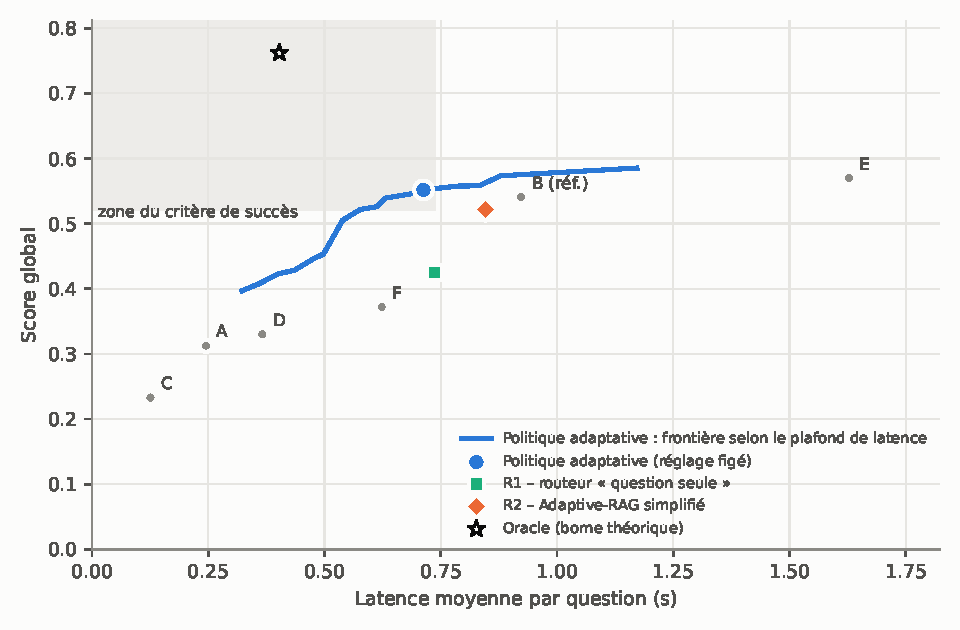
\includegraphics[width=0.78\linewidth]{figures/partie4_qualite_cout.pdf}
\caption{Compromis qualité--latence sur le jeu de développement. La courbe bleue indique, pour chaque
plafond de latence, le meilleur score que peut atteindre la politique ; le point bleu correspond au
réglage figé. La zone grisée est celle du critère de succès.}
\label{fig:dev}
\end{figure}

Sur le jeu de développement, la politique remplissait le critère principal, avec un léger gain de score
et 23~\% de latence en moins, et elle devançait les deux routeurs. Deux signaux d'alerte étaient
néanmoins visibles. La validation croisée estimait une perte de 2,1 points, juste à la limite du
critère. Surtout, les questions simples perdaient quatorze points, en échange d'un gain de vingt-deux
points sur les questions non couvertes : le critère de robustesse n'était déjà pas satisfait.

%======================================================================
\section{Évaluation finale}\label{sec:final}
%======================================================================

\subsection{Conditions d'exécution}

Une fois la politique figée et publiée, nous avons exécuté les six stratégies fixes et la politique sur
les 450 questions du jeu de test, en trois passes complètes. Dans chaque passe, l'ordre des méthodes
était tiré au hasard, afin de répartir l'effet de l'échauffement de la machine ; la latence retenue pour
chaque question est la médiane des trois passes. La politique a été exécutée réellement, de bout en
bout. Les routeurs R1 et R2, entraînés sur l'ensemble du jeu de développement, ont été appliqués aux
sorties du test. L'énergie a été mesurée pendant toute l'évaluation, soit plus de 30\,000 relevés, pour
une puissance au repos de 2,7~W.

Deux contrôles attestent la solidité de l'exécution. Les réponses sont identiques d'une passe à l'autre
pour toutes les méthodes. Et la politique exécutée reproduit exactement sa simulation : même score sur
chacune des questions, même latence moyenne à un millième de seconde près.

\subsection{Résultats}

\begin{table}[H]
\centering\small\setlength{\tabcolsep}{4pt}
\begin{tabular}{l c c c c c c c}
\toprule
Méthode & Score & IC 95~\% & Écart à B & Latence & P95 & Couv. & Risque \\
\midrule
A -- grand, sans RAG & 0,310 & [0,269 ; 0,351] & $-22{,}7$ & 0,27~s & 0,52~s & 0,45 & 0,76 \\
\textbf{B -- grand, 3 passages (réf.)} & \textbf{0,537} & [0,494 ; 0,581] & -- & \textbf{0,87~s} & 1,26~s & 0,73 & 0,42 \\
C -- petit, sans RAG & 0,223 & [0,187 ; 0,261] & $-31{,}4$ & 0,13~s & 0,25~s & 0,51 & 0,93 \\
D -- petit, 3 passages & 0,414 & [0,372 ; 0,457] & $-12{,}3$ & 0,35~s & 0,53~s & 0,88 & 0,57 \\
E -- grand, 6 passages & 0,567 & [0,523 ; 0,610] & $+3{,}0$ & 1,57~s & 2,23~s & 0,75 & 0,40 \\
F -- petit, 6 passages & 0,398 & [0,357 ; 0,440] & $-13{,}9$ & 0,61~s & 0,87~s & 0,94 & 0,60 \\
\midrule
R1 -- question seule & 0,489 & [0,445 ; 0,534] & $-4{,}7$ & 0,74~s & 1,61~s & 0,68 & 0,48 \\
R2 -- Adaptive-RAG simplifié & 0,517 & [0,473 ; 0,561] & $-2{,}0$ & 0,82~s & 1,39~s & 0,68 & 0,44 \\
\textbf{Politique adaptative} & \textbf{0,550} & [0,505 ; 0,594] & $\mathbf{+1{,}3}$ & \textbf{0,79~s} & 1,38~s & 0,64 & \textbf{0,40} \\
\midrule
\textit{Oracle} & \textit{0,797} & [0,762 ; 0,831] & $+26{,}0$ & \textit{0,36~s} & 1,09~s & 0,64 & 0,18 \\
\bottomrule
\end{tabular}
\caption{Résultats sur le jeu de test (450 questions). La latence est la moyenne, sur les questions, de
la médiane des trois passes.}
\label{tab:resultats}
\end{table}

\begin{figure}[H]
\centering
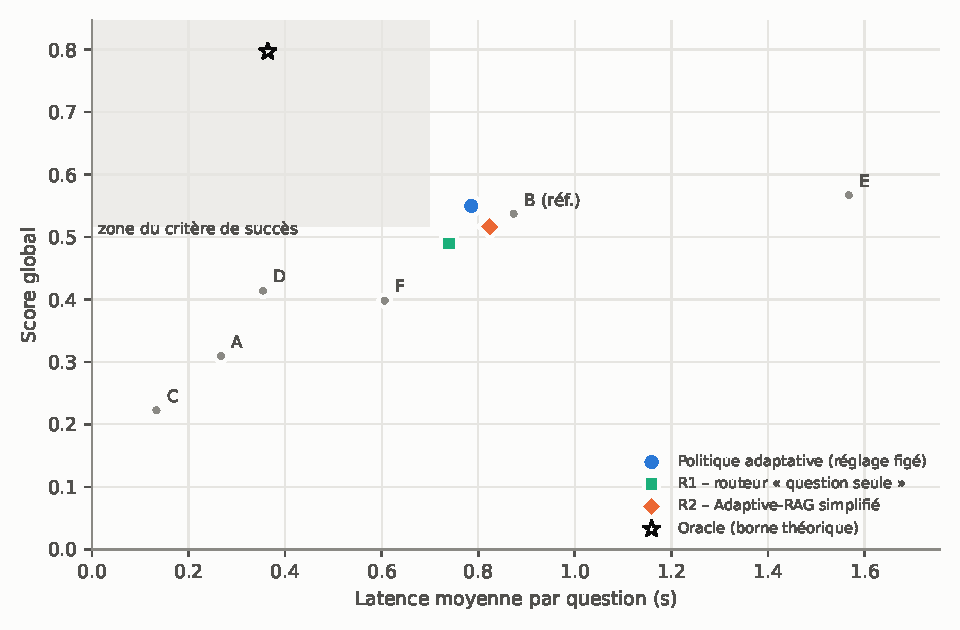
\includegraphics[width=0.78\linewidth]{figures/partie5_qualite_cout.pdf}
\caption{Compromis qualité--latence sur le jeu de test. La politique (en bleu) se situe au-dessus de B,
mais à droite de la zone du critère de succès.}
\label{fig:test}
\end{figure}

La politique obtient le meilleur score de toutes les méthodes réalisables à l'exception de E, qui est
deux fois plus lente. Elle devance B d'un peu plus d'un point, fait moins d'erreurs lorsqu'elle répond,
et dépasse nettement les deux routeurs. Mais sa latence moyenne n'est inférieure que de 10~\% à celle de
B.

\subsection{Verdict}

\begin{table}[H]
\centering\small
\begin{tabularx}{\linewidth}{Y >{\centering\arraybackslash}p{5.6cm} c}
\toprule
Critère & Mesure & Atteint \\
\midrule
Latence moyenne réduite d'au moins 20~\% & $-10{,}1$~\% (0,786 contre 0,873~s) & \non \\
Perte de score d'au plus 2~points & gain de 1,3 point & \oui \\
Non-infériorité (borne haute de l'IC de la perte sous 2~points) & $[-4{,}1\,;\,+1{,}6]$ & \oui \\
\textbf{Critère principal} & & \non \\
\midrule
Risque inférieur à B & 0,395 contre 0,421 & \oui \\
Meilleur score que R1 et R2 & 0,550 contre 0,489 et 0,517 & \oui \\
Aucune catégorie ne perd plus de 5~points & simple $-7{,}6$ ; complexe $-3{,}3$ ; non couverte $+14{,}7$ & \non \\
\bottomrule
\end{tabularx}
\caption{Verdict sur les critères pré-enregistrés.}
\label{tab:verdict}
\end{table}

Le verdict est donc nuancé. La qualité est préservée, la non-infériorité est démontrée, la fiabilité
s'améliore et les deux routeurs de référence sont battus. Mais l'économie de latence n'atteint que la
moitié de l'objectif, et les questions simples paient le prix de l'abstention. L'hypothèse principale,
dans la forme où nous l'avions enregistrée, est rejetée.

\subsection{Analyse par catégorie}

\begin{table}[H]
\centering\small
\begin{tabular}{l c c c}
\toprule
Méthode & Simple & Complexe & Non couverte \\
\midrule
B -- référence & 0,737 & 0,468 & 0,407 \\
E -- grand, 6 passages & 0,730 & 0,537 & 0,433 \\
R1 & 0,562 & 0,453 & 0,453 \\
R2 & 0,635 & 0,455 & 0,460 \\
\textbf{Politique adaptative} & 0,661 ($-7{,}6$) & 0,435 ($-3{,}3$) & \textbf{0,553} ($+14{,}7$) \\
\textit{Oracle} & 0,842 & 0,682 & 0,867 \\
\bottomrule
\end{tabular}
\caption{Score par catégorie sur le jeu de test (150 questions chacune). Entre parenthèses, l'écart à B
en points.}
\label{tab:categories}
\end{table}

La politique échange de la qualité sur les questions qui ont une réponse contre de la fiabilité sur
celles qui n'en ont pas. Sur les 450 questions, elle a déclenché 66 abstentions précoces et fait
répondre le grand modèle 359 fois avec trois passages et 25 fois avec six ; 98 de ces réponses ont
ensuite été remplacées par une abstention finale. Les abstentions précoces frappent surtout les
questions non couvertes, ce qui est le but recherché, mais aussi 18 questions simples et 12 complexes :
un score BM25 faible ne signifie pas toujours que la réponse est absente.

\subsection{Ablations}

\begin{table}[H]
\centering\small
\begin{tabular}{l c c c c}
\toprule
& \multicolumn{2}{c}{\textbf{Test}} & \multicolumn{2}{c}{\textbf{Développement}} \\
\textbf{Variante} (chacune réglée sur le développement) & Score & Latence & Score & Latence \\
\midrule
\textbf{Politique complète} & \textbf{0,550} & 0,79~s & 0,552 & 0,71~s \\
Sans recherche adaptative (toujours 3 passages) & 0,547 & 0,74~s & 0,548 & 0,68~s \\
Sans abstention finale & 0,547 & 0,79~s & 0,546 & 0,71~s \\
Sans abstention précoce (cascade petit $\to$ grand) & 0,464 & 0,64~s & 0,395 & 0,70~s \\
Sans aucune abstention & 0,457 & 0,64~s & 0,389 & 0,70~s \\
\bottomrule
\end{tabular}
\caption{Ablations : chaque composante est retirée et la politique est réglée à nouveau.}
\label{tab:ablations}
\end{table}

Les ablations désignent clairement la composante décisive : sans abstention précoce, la politique perd
près de neuf points sur le test. La recherche adaptative et l'abstention finale, elles, n'apportent
chacune que trois dixièmes de point, ce qui reste dans le bruit statistique. Sur le test, s'en tenir
toujours à trois passages aurait même été plus rapide, pour un score équivalent.

\subsection{Énergie}

\begin{table}[H]
\centering\small
\begin{tabular}{l c c c}
\toprule
Méthode & Énergie par question & Écart à B & Puissance moyenne \\
\midrule
C -- petit, sans RAG & 1,8~J & $-90$~\% & 16,4~W \\
A -- grand, sans RAG & 3,9~J & $-80$~\% & 17,0~W \\
D -- petit, 3 passages & 7,3~J & $-62$~\% & 23,2~W \\
F -- petit, 6 passages & 13,5~J & $-30$~\% & 24,9~W \\
\textbf{Politique adaptative} & \textbf{17,5~J} & $\mathbf{-9}$~\% & 24,8~W \\
B -- grand, 3 passages (réf.) & 19,3~J & -- & 24,7~W \\
E -- grand, 6 passages & 37,7~J & $+95$~\% & 26,4~W \\
\bottomrule
\end{tabular}
\caption{Énergie de la puce (processeur, GPU et moteur neuronal) par question sur le test, moyenne des
trois passes.}
\label{tab:energie}
\end{table}

La puissance appelée varie peu d'une méthode à l'autre, entre 16 et 26~W. L'énergie suit donc
essentiellement la durée du calcul, c'est-à-dire le nombre de tokens traités, et l'économie de la
politique ($-9$~\%) reflète sa réduction de latence. On notera au passage que doubler le nombre de
passages double presque l'énergie, pour trois points de score.

\subsection{Du développement au test}

\begin{table}[H]
\centering\small
\begin{tabular}{l c c c c}
\toprule
& \multicolumn{2}{c}{Développement (180)} & \multicolumn{2}{c}{Test (450)} \\
Méthode & Score & Latence & Score & Latence \\
\midrule
B -- référence & 0,541 & 0,92~s & 0,537 & 0,87~s \\
Politique adaptative & 0,552 & 0,71~s ($-23$~\%) & 0,550 & 0,79~s ($-10$~\%) \\
R1 & 0,425 & 0,74~s & 0,489 & 0,74~s \\
R2 & 0,522 & 0,85~s & 0,517 & 0,82~s \\
Oracle & 0,762 & 0,40~s & 0,797 & 0,36~s \\
\midrule
Abstentions précoces & \multicolumn{2}{c}{45 / 180 (25~\%)} & \multicolumn{2}{c}{66 / 450 (15~\%)} \\
\bottomrule
\end{tabular}
\caption{Comparaison entre jeu de développement et jeu de test.}
\label{tab:dev-test}
\end{table}

C'est en comparant les deux jeux que l'échec s'éclaire. La qualité s'est remarquablement bien
généralisée : 0,550 sur le test, mieux même que les 0,520 prévus par la validation croisée. Le gain de
latence, en revanche, s'est réduit de moitié. Le seuil d'abstention précoce, réglé sur soixante
questions par catégorie, écartait un quart des questions de développement, mais seulement 15~\% des
questions de test. L'écart représente environ trois erreurs-types, ce qui l'attribue à la variabilité
d'un trop petit échantillon de réglage. Moins d'abstentions précoces, c'est davantage d'appels au grand
modèle, et donc une latence qui se rapproche de celle de B.

%======================================================================
\section{Discussion}\label{sec:discussion}
%======================================================================

\subsection{Retour sur les hypothèses}

La première hypothèse est rejetée. Aucun signal calculé avant génération n'a permis d'envoyer des
questions au petit modèle sans perte : R1 perd entre cinq et douze points selon le jeu, et la politique
réglée a écarté le petit modèle. La deuxième n'est pas confirmée. La politique fait moins d'erreurs que
B, mais la confiance du modèle n'ajoute presque rien à la preuve : sans abstention finale, le score et
le risque sont pratiquement inchangés. La troisième est partiellement confirmée. Aucune autre méthode
n'est à la fois plus précise et plus rapide que la politique, qui domine B ; mais son avantage de coût
reste modeste. La quatrième, enfin, est pleinement confirmée : sept points perdus sur les questions
simples, quinze gagnés sur les questions non couvertes. Une moyenne seule aurait masqué ce compromis.

\subsection{Ce que nous retenons}

Le premier enseignement est que, dans notre cadre, \emph{ce que la recherche a trouvé renseigne mieux
que la question elle-même}. À latence comparable, la politique devance R1 de six points et R2 de trois.
Ce résultat contraste avec celui de \citet{li2026beyond}, pour qui les signaux issus de la recherche
n'améliorent pas de façon fiable un routeur fondé sur la requête. La différence tient peut-être au rôle
que nous donnons à ce signal : nous ne l'utilisons pas pour choisir entre plusieurs façons de répondre,
mais pour décider de ne pas répondre du tout.

Le deuxième enseignement est que \emph{l'abstention rend l'adaptation rentable}. Ne rien générer
lorsque la preuve est faible économise du calcul et évite des erreurs dans le même mouvement. C'est la
seule composante dont l'effet dépasse nettement le bruit. Le troisième concerne le petit modèle, qui n'a
pas trouvé sa place : sa confiance ne signale ses erreurs que modérément, et chaque escalade fait payer
deux générations. Le dernier est une invitation à poursuivre. L'oracle atteint près de 0,80 en 0,36~s :
les bons choix existent, et la difficulté est de les prédire.

\subsection{Portée pratique}

Pour qui déploie un assistant local, ces résultats suggèrent une règle simple et peu risquée : mesurer la
suffisance des preuves, qui ne coûte rien, et s'abstenir lorsque les documents ne contiennent
manifestement pas les termes de la question. On conserve ainsi la qualité de la configuration complète,
on réduit les réponses fausses, et l'on gagne un peu de temps et d'énergie. Il faut toutefois régler le
seuil sur un échantillon représentatif, ou mieux, l'exprimer comme une proportion de questions, faute
de quoi le gain de temps devient imprévisible.

%======================================================================
\section{Points faibles et pistes d'amélioration}\label{sec:faiblesses}
%======================================================================

Une évaluation honnête doit dire ce qui n'a pas marché et pourquoi. Nous présentons ici les faiblesses
de l'étude, de la plus lourde de conséquences à la plus secondaire, en proposant pour chacune une voie
d'amélioration. Le tableau~\ref{tab:faiblesses} les récapitule.

\subsection{Faiblesses de la méthode}

\paragraph{Des seuils absolus réglés sur un petit échantillon.} C'est la cause directe de l'échec du
critère principal. Un seuil fixé sur une valeur absolue de la preuve, à partir de soixante questions par
catégorie, ne déclenche pas la même proportion d'abstentions sur un autre jeu de questions, et la
validation croisée, menée sur le même petit échantillon, ne pouvait pas le révéler. Plusieurs remèdes
sont possibles et se combinent : exprimer le seuil comme un quantile ou un budget (« s'abstenir sur les
$x$~\% de questions aux preuves les plus faibles »), ce qui garantit le taux d'abstention et donc la
latence ; le calibrer par une méthode conforme, qui offre des garanties de risque sans hypothèse sur la
distribution \citep{hao2026racer} ; régler sur au moins cinq cents questions ; et fonder la marge de
sécurité sur la variabilité mesurée par bootstrap plutôt que sur une valeur fixée à l'avance.

\paragraph{Des questions simples sacrifiées.} L'abstention précoce écarte aussi des questions qui ont
une réponse, parce qu'une reformulation ou un synonyme suffit à faire chuter le score lexical. La
couverture passe ainsi de 0,73 à 0,64. Un juge de suffisance plus fin, tel un re-classeur de type
\emph{cross-encoder} ou un petit modèle d'inférence, dans l'esprit de Corrective RAG
\citep{yan2024crag} et de Tiny-Critic RAG \citep{wu2026tinycritic}, devrait réduire ces faux négatifs.
Combiner preuves lexicale et dense irait dans le même sens, de même qu'une contrainte explicite par
catégorie lors du réglage.

\paragraph{Des signaux de confiance faibles.} Aucun signal ne dépasse une AUC de 0,74, et l'abstention
finale n'apporte presque rien. La probabilité des tokens d'une réponse de quelques mots renseigne mal sur
sa justesse. L'entropie sémantique \citep{kuhn2023semantic} ou la cohérence entre quelques réponses
échantillonnées seraient plus informatives ; pour en contenir le coût, on pourrait les réserver aux cas
limites. Une sonde entraînée sur les états internes du modèle \citep{kadavath2022know} est une autre
piste.

\paragraph{Une recherche adaptative sans effet.} Passer de trois à six passages ne concerne que 6~\% des
questions et n'apporte rien de mesurable. Or les questions complexes n'ont qu'un rappel@3 de 0,37 : le
problème n'est pas le nombre de passages, mais la recherche elle-même. Décomposer les questions à
plusieurs étapes, déclencher une recherche itérative lorsque le modèle hésite
\citep{jiang2023flare,su2024dragin} et compresser le contexte pour réduire le coût des passages
supplémentaires \citep{arefeen2024leancontext} seraient plus prometteurs.

\paragraph{Un petit modèle inutilisé.} La politique finale ne recourt qu'à un seul modèle, si bien que
la dimension « choix du modèle » de notre problématique n'est pas réellement exploitée. Un petit modèle
plus performant ou spécialisé dans l'extraction pourrait changer la donne. On peut aussi lui confier un
rôle moins exigeant, comme la reformulation de requêtes, ou recourir au décodage spéculatif, où le petit
modèle accélère le grand sans modifier ses réponses.

\paragraph{Une latence de queue dégradée et un écart persistant à l'oracle.} Le 95\textsuperscript{e}
centile de la latence de la politique (1,38~s) dépasse celui de B (1,26~s), à cause des réponses à six
passages ; il faudrait l'intégrer à l'objectif de réglage. Quant à l'écart de vingt-cinq points avec
l'oracle, seul un routeur appris combinant question, preuve et confiance, entraîné sur bien plus de
données, pourrait espérer le réduire sensiblement.

\subsection{Faiblesses du protocole}

\paragraph{Un benchmark construit et restreint.} Les questions sont en anglais, tirées de deux jeux
académiques, et interrogent un corpus fermé de 3\,293 passages. Les questions non couvertes sont des
questions adverses de SQuAD 2.0, rédigées pour ressembler aux passages, ce qui ne reflète pas l'usage
réel. La catégorie des questions ambiguës n'a pas été constituée. Ajouter MuSiQue
\citep{trivedi2022musique} et le CRAG Benchmark \citep{yang2024cragbench}, un corpus réel en français et
une cinquantaine de questions ambiguës annotées à la main élargirait considérablement la portée des
conclusions.

\paragraph{Une métrique lexicale.} Le F1 pénalise les réponses justes formulées autrement, qu'il
s'agisse d'une paraphrase, d'un synonyme ou d'une date écrite différemment. Un juge sémantique, modèle
d'inférence ou LLM évaluateur, validé sur un échantillon annoté à la main, donnerait une image plus
fidèle.

\paragraph{Une puissance statistique limitée.} Avec 450 questions, l'intervalle de confiance du score
s'étend sur environ quatre points et demi de part et d'autre de l'estimation : un écart de deux points,
le seuil même de notre critère, n'est pas détectable avec certitude. Un jeu de test d'au moins 1\,500
questions serait nécessaire.

\paragraph{Un seul matériel, une seule mesure.} Toutes les mesures proviennent d'un même appareil, avec
un seul moteur d'inférence et une seule quantification, et l'énergie est celle de la puce, non la
consommation au mur. Répliquer l'étude sur GPU et avec \texttt{llama.cpp}, mesurer au wattmètre et
rapporter la mémoire consolideraient les conclusions sur le coût.

\paragraph{Une conception explorée sur le développement.} Deux conceptions ont été essayées avant de
figer la politique. C'est documenté, mais cela accroît le risque de sur-ajustement au jeu de
développement. Il faudrait à l'avenir pré-enregistrer aussi la famille de politiques envisagées, et
évaluer toute amélioration sur un jeu de test neuf, celui-ci étant désormais consommé.

\paragraph{Une revue à approfondir.} Notre état de l'art s'appuie largement sur les résumés des
articles. Une lecture intégrale des travaux les plus proches (Adaptive-RAG,
\citealp{moskvoretskii2025adaptive}, RAGRouter-Bench, RACER et \citealp{li2026beyond}) est nécessaire pour
confirmer le positionnement proposé au tableau~\ref{tab:positionnement}.

\begin{table}[H]
\centering\small
\begin{tabularx}{\linewidth}{Y Y c}
\toprule
Faiblesse & Amélioration principale & Priorité \\
\midrule
Seuils absolus, petit jeu de réglage & Seuils en quantiles ou budget, calibration conforme, au moins 500 questions & Haute \\
Perte sur les questions simples & Juge de suffisance léger, contrainte par catégorie & Haute \\
Puissance statistique limitée & Jeu de test d'au moins 1\,500 questions & Haute \\
Signaux de confiance faibles & Cohérence entre échantillons sur les cas limites & Moyenne \\
Recherche adaptative sans effet & Décomposition des questions à plusieurs étapes & Moyenne \\
Benchmark restreint & MuSiQue, CRAG, corpus français, questions ambiguës & Moyenne \\
Métrique lexicale & Juge sémantique validé & Moyenne \\
Petit modèle inutilisé & Autre petit modèle, décodage spéculatif & Moyenne \\
Revue fondée sur les résumés & Lecture intégrale des travaux proches & Moyenne \\
Latence de queue & 95\textsuperscript{e} centile dans l'objectif de réglage & Basse \\
Écart à l'oracle & Routeur appris multi-signaux & Basse \\
Matériel unique & Réplication sur GPU, wattmètre & Basse \\
Exploration sur le développement & Pré-enregistrer la famille de politiques & Basse \\
\bottomrule
\end{tabularx}
\caption{Synthèse des points faibles et des améliorations proposées.}
\label{tab:faiblesses}
\end{table}

%======================================================================
\section{Conclusion}\label{sec:conclusion}
%======================================================================

Nous sommes partis d'une question pratique : comment un assistant qui tourne sur une machine
personnelle peut-il dépenser ses ressources avec discernement, en donnant à chaque question l'effort
qu'elle mérite ? Pour y répondre, nous avons construit un benchmark et un protocole dont les critères de
succès étaient fixés d'avance, établi des références solides, puis conçu une politique qui décide
ensemble du modèle, du nombre de passages et de l'abstention, à partir de la suffisance des preuves et
de la confiance du modèle.

Le résultat est en demi-teinte, et nous le rapportons comme tel. Sur le jeu de test, la politique
préserve la qualité de la configuration de référence, commet moins d'erreurs et dépasse deux routeurs
inspirés de la littérature. Mais elle ne réduit la latence que de 10~\% et l'énergie de 9~\%, au lieu
des 20~\% espérés. Nous en connaissons la cause : un seuil absolu, réglé sur un échantillon trop petit,
qui s'est moins souvent déclenché sur des questions nouvelles.

Deux idées nous semblent survivre à ce résultat. Sur une machine locale, la qualité des preuves
retrouvées est un guide plus sûr que la formulation de la question. Et savoir s'abstenir est ce qui
permet d'économiser sans renoncer à la fiabilité. La suite du travail consiste à rendre ce levier
stable : exprimer l'abstention comme un budget calibré, mieux juger la suffisance des preuves, et
valider le tout sur un jeu de test plus vaste et entièrement neuf.

\paragraph{Reproductibilité.} Le code, le benchmark et les empreintes de ses données, les configurations
figées (étiquettes \texttt{protocole-v1.0} et \texttt{politique-v1.0}), les sorties brutes des trois
passes et les mesures d'énergie sont publiés dans le dépôt indiqué en première page.

\bibliographystyle{plainnat}
\bibliography{references}

\end{document}
